% !TEX root = ../../presentation.tex
% Core

\begin{slide}{MemoryValue}
\scalebox{1.0}{
  \begin{tabular}{l} \pause
    \texttt{std::bitset}\\\\ \pause
    \texttt{boost::dynamic\_bitset}\\\\ \pause
    \texttt{std::vector\textless uint8\textgreater}\\\\ \pause
    \texttt{std::vector}\textless bool\textgreater\\\\ \pause
  \end{tabular}
  }
\end{slide}

\begin{slide}{MemoryValue}
    {\large
    Lesen und Schreiben einzelner Bits\\
    }
    \vspace{1cm}
\scalebox{1.0}{
  \begin{tabular}{l|c}
    \texttt{std::bitset} & $\checkmark$ \\
    \texttt{boost::dynamic\_bitset} & $\checkmark$ \\
    \texttt{std::vector\textless uint8\textgreater} & $\times$ \\
    \texttt{std::vector}\textless bool\textgreater & $\checkmark$ \\
  \end{tabular}
 }
\end{slide}

\begin{slide}{MemoryValue}
{\large
    Lesen und Schreiben einzelner Bytes\\
}
\vspace{1cm}
\scalebox{1.0}{
  \begin{tabular}{l|c}
    \texttt{std::bitset} & $\times$ \\
    \texttt{boost::dynamic\_bitset} & $\times$ \\
    \texttt{std::vector\textless uint8\textgreater} & $\checkmark$ \\
    \texttt{std::vector}\textless bool\textgreater & $\times$ \\
  \end{tabular}
  }
\end{slide}

\begin{slide}{MemoryValue}
{\large
    Lesen und Schreiben einzelner Teilabschnitten\\
}
\vspace{1cm}
\scalebox{1.0}{
  \begin{tabular}{l|c}
    \texttt{std::bitset} & $\times$ \\
    \texttt{boost::dynamic\_bitset} & $\times$ \\
    \texttt{std::vector\textless uint8\textgreater} & $\checkmark$ \\
    \texttt{std::vector}\textless bool\textgreater & $\checkmark$ \\
  \end{tabular}
  }
\end{slide}

\begin{slide}{MemoryValue}
{\large
    Größe kann dynamisch festgelegt werden\\
}
\vspace{1cm}
\scalebox{1.0}{
  \begin{tabular}{l|c}
    \texttt{std::bitset} & $\times$ \\
    \texttt{boost::dynamic\_bitset} & $\checkmark$ \\
    \texttt{std::vector\textless uint8\textgreater} & $\checkmark$ \\
    \texttt{std::vector}\textless bool\textgreater & $\checkmark$ \\
  \end{tabular}
  }
\end{slide}

\begin{slide}{MemoryValue}
\scalebox{0.65}{
  \begin{tabular}{l|cccc}
    \texttt{std::bitset} & $\checkmark$ & $\times$ & $\times$ & $\times$ \\\\
    \texttt{boost::dynamic\_bitset} & $\checkmark$ & $\times$ & $\times$ & $\checkmark$ \\\\
    \texttt{std::vector\textless uint8\textgreater} & $\times$ & $\checkmark$ & $\checkmark$ & $\checkmark$ \\\\
    \texttt{std::vector}\textless bool\textgreater & $\checkmark$ & $\times$ & $\checkmark$ & $\checkmark$ \\\\
    \texttt{MemoryValue} & $\checkmark$ & $\checkmark$ & $\checkmark$ & $\checkmark$ \\\\
  \end{tabular}
  }
\end{slide}

\begin{slide}{Konvertierungen}
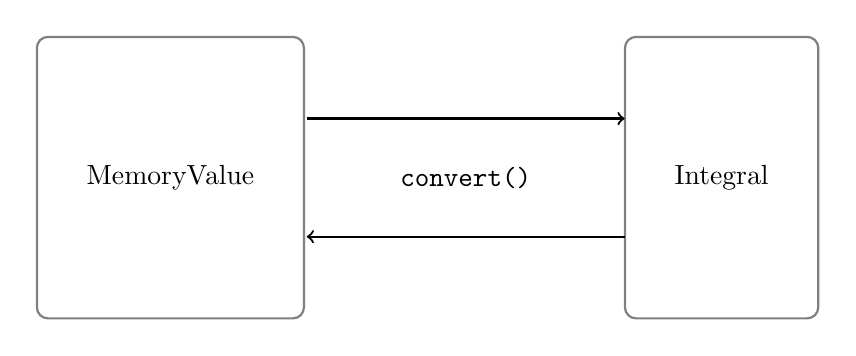
\begin{tikzpicture} [thick]
    \tikzset{block/.style={%
      draw,%
      rectangle,%
      rounded corners,%
      text width=2cm,%
      text height=0.45cm}%
    };
\tikzset{smallblock/.style={block, text width=1.5cm, text height=0.3cm}};

\node (memoryValue) at (-3.5, 0) {MemoryValue};
\node (aboveMV) at (-1.9, 0.75) {};
\node (belowMV) at (-1.9, -0.75) {};

%memory value outline
\path (memoryValue.west |- memoryValue.north)+(-0.5,1.5) node (a1) {};
\path (memoryValue.east |- memoryValue.south)+(0.5,-1.5) node (a2) {};
\path[rounded corners, draw=black!50, thick] (a1) rectangle (a2);


\node (integral) at (3.5, 0) {Integral};
\node (aboveI) at (2.4, 0.75) {};
\node (belowI) at (2.4, -0.75) {};

%memory value outline
\path (integral.west |- integral.north)+(-0.5,1.5) node (a1) {};
\path (integral.east |- integral.south)+(0.5,-1.5) node (a2) {};
\path[rounded corners, draw=black!50, thick] (a1) rectangle (a2);

\draw [->] (aboveMV) -- (aboveI);
\draw [<-] (belowMV) -- (belowI);

%text between arrows
\node (convert) at (0.25, 0) {\texttt{convert()}};

\end{tikzpicture}
\end{slide}

\begin{slide}{RegisterSet}
\begin{tikzpicture}

  % pseudo element for centering
  \node (center) {};

  \node (eax)
    [font=\scriptsize, draw=black, rounded corners, align=center, minimum height=0.68cm, minimum width=3cm, above left=0.5cm and 3cm of center]
    {\texttt{EAX}};
  \node (ebx)
    [font=\scriptsize, draw=black, rounded corners, align=center, minimum height=0.68cm, minimum width=3cm, above left=-1.5cm and 3cm of center]
    {\texttt{EBX}};

  \node (mapEax)
    [font=\scriptsize, draw=black,  align=center, minimum height=0.5cm, minimum width=2cm, above left=1.35cm and 7cm of center]
    {\texttt{"}\texttt{eax"[0,31]}}
      edge [->, out=0, in=180] (eax);
  \node (mapAx)
    [font=\scriptsize, draw=black,  align=center, minimum height=0.5cm, minimum width=2cm, above left=0.85cm and 7cm of center]
    {\texttt{"}\texttt{ax"[0,15]}}
      edge [->, out=0, in=180] (eax);
  \node (mapAl)
    [font=\scriptsize, draw=black,  align=center, minimum height=0.5cm, minimum width=2cm, above left=0.35cm and 7cm of center]
    {\texttt{"}\texttt{al"[0,7]}}
      edge [->, out=0, in=180] (eax);
  \node (mapAh)
    [font=\scriptsize, draw=black,  align=center, minimum height=0.5cm, minimum width=2cm, above left=-0.15cm and 7cm of center]
    {\texttt{"}\texttt{ah"[8,15]}}
      edge [->, out=0, in=180] (eax);
  \node (mapEbx)
    [font=\scriptsize, draw=black,  align=center, minimum height=0.5cm, minimum width=2cm, above left=-0.65cm and 7cm of center]
    {\texttt{"}\texttt{ebx"[0,31]}}
      edge [->, out=0, in=180] (ebx);
  \node (mapBx)
    [font=\scriptsize, draw=black,  align=center, minimum height=0.5cm, minimum width=2cm, above left=-1.15cm and 7cm of center]
    {\texttt{"}\texttt{bx"[0,15]}}
      edge [->, out=0, in=180] (ebx);
  \node (mapBl)
    [font=\scriptsize, draw=black,  align=center, minimum height=0.5cm, minimum width=2cm, above left=-1.65cm and 7cm of center]
    {\texttt{"}\texttt{bl"[0,7]}}
      edge [->, out=0, in=180] (ebx);
  \node (mapBh)
    [font=\scriptsize, draw=black,  align=center, minimum height=0.5cm, minimum width=2cm, above left=-2.15cm and 7cm of center]
    {\texttt{"}\texttt{bh"[8,15]}}
      edge [->, out=0, in=180] (ebx);

  \node (eaxUpdate)
    [font=\scriptsize, draw=black, align=center, minimum height=1.70cm, minimum width=0.8cm, above left=0cm and -1cm of center, rounded corners]
    {\begin{tabular}{c}
      \texttt{"}\texttt{eax"} \\
      \texttt{"}\texttt{ax"} \\
      \texttt{"}\texttt{al"} \\
      \texttt{"}\texttt{ah"} \\
    \end{tabular}};
  \node (ebxUpdate)
    [font=\scriptsize, draw=black, align=center, minimum height=1.70cm, minimum width=0.8cm, above left=-2cm and -1cm of center, rounded corners]
    {\begin{tabular}{c}
      \texttt{"}\texttt{ebx"} \\
      \texttt{"}\texttt{bx"} \\
      \texttt{"}\texttt{bl"} \\
      \texttt{"}\texttt{bh"} \\
    \end{tabular}};

  \draw [->] (eax) -- (eaxUpdate);
  \draw [->] (ebx) -- (ebxUpdate);

\end{tikzpicture}
\end{slide}
